\chapter*{Dodatak: Prikaz aktivnosti grupe}
		\addcontentsline{toc}{chapter}{Dodatak: Prikaz aktivnosti grupe}
		
		\section*{Dnevnik sastajanja}
		
		\textbf{\textit{Kontinuirano osvježavanje}}\\
		
	
		
		\begin{packed_enum}
			\item  sastanak
			
			\item[] \begin{packed_item}
				\item Datum: 4. listopada 2020.
				\item Prisustvovali: F. Hrabar, I. Mihovilović, Z. Protulipac, Z. Pećanić, T. Likakur, J. Vujević, M. Kukelšćak
				\item Teme sastanka:
				\begin{packed_item}
					\item  organizacija grupe
					\item  raspodjela posla
				\end{packed_item}
			\end{packed_item}
			
			\item  sastanak
			\item[] \begin{packed_item}
				\item Datum: 15. listopada 2020.
				\item Prisustvovali: F. Hrabar, I. Mihovilović, Z. Protulipac, Z. Pećanić, T. Likakur, J. Vujević, M. Kukelšćak
				\item Teme sastanka:
				\begin{packed_item}
					\item  odabir programske potpore koja će se koristiti
					\item  izgled i dizajn aplikacije
				\end{packed_item}
			\end{packed_item}
			
			\item  sastanak
			\item[] \begin{packed_item}
				\item Datum: 2. 11. 2020.
				\item Prisustvovali: F. Hrabar, I. Mihovilović, Z. Protulipac, Z. Pećanić, T. Likakur, J. Vujević, M. Kukelšćak
				\item Teme sastanka:
				\begin{packed_item}
					\item  izvedba backenda i povezivanje s frontendom (json)
					\item  povezivanje git - Heroku
				\end{packed_item}
			\end{packed_item}
			%
			\item  sastanak
			\item[] \begin{packed_item}
				\item Datum: 8. 11. 2020.
				\item Prisustvovali: F. Hrabar, I. Mihovilović, Z. Protulipac, Z. Pećanić, T. Likakur, J. Vujević, M. Kukelšćak
				\item Teme sastanka:
				\begin{packed_item}
					\item  izvedba frontenda
					\item  json i povezivanje backend-frontend
				\end{packed_item}
			\end{packed_item}
			%
			\item  sastanak
			\item[] \begin{packed_item}
				\item Datum: 20. 11. 2020.
				\item Prisustvovali: F. Hrabar, I. Mihovilović, Z. Protulipac, Z. Pećanić, T. Likakur, J. Vujević, M. Kukelšćak
				\item Teme sastanka:
				\begin{packed_item}
					\item  daljnja podjela posla
					\item  backend
				\end{packed_item}
			\end{packed_item}
			%
			\item  sastanak
			\item[] \begin{packed_item}
				\item Datum: 28. 11. 2020.
				\item Prisustvovali: F. Hrabar, I. Mihovilović, Z. Protulipac, Z. Pećanić, T. Likakur, J. Vujević, M. Kukelšćak
				\item Teme sastanka:
				\begin{packed_item}
					\item  frontend i json
					\item  cart
					\item  dodatci u bazi
					
				\end{packed_item}
			\end{packed_item}
		
			\item  sastanak
			\item[] \begin{packed_item}
				\item Datum: 6. 12. 2020.
				\item Prisustvovali: F. Hrabar, I. Mihovilović, Z. Protulipac, Z. Pećanić, T. Likakur, J. Vujević, M. Kukelšćak
				\item Teme sastanka:
				\begin{packed_item}
					\item  cart
					\item  backend
					\item  podjela posla tijekom praznika
					
					
				\end{packed_item}
			\end{packed_item}
			%
			\item  sastanak
			\item[] \begin{packed_item}
				\item Datum: 12. 12. 2020.
				\item Prisustvovali: F. Hrabar, I. Mihovilović, Z. Protulipac, Z. Pećanić, T. Likakur, J. Vujević, M. Kukelšćak
				\item Teme sastanka:
				\begin{packed_item}
					\item  uloge admina
				
					
				\end{packed_item}
			\end{packed_item}
		
			\item  sastanak
			\item[] \begin{packed_item}
				\item Datum: 18. 12. 2020.
				\item Prisustvovali: F. Hrabar, I. Mihovilović, Z. Protulipac, Z. Pećanić, T. Likakur, J. Vujević, M. Kukelšćak
				\item Teme sastanka:
				\begin{packed_item}
					\item  podjela posla do kraja
					\item dokumentacija - dijagrami u 2. ciklusu
				
					
				\end{packed_item}
			\end{packed_item}
		
			\item  sastanak
			\item[] \begin{packed_item}
				\item Datum: 27. 12. 2020.
				\item Prisustvovali: F. Hrabar, I. Mihovilović, Z. Protulipac, Z. Pećanić, T. Likakur, J. Vujević, M. Kukelšćak
				\item Teme sastanka:
				\begin{packed_item}
					\item  backend
					\item  vodeni žig
				
					
				\end{packed_item}
			\end{packed_item}
		
			\item  sastanak
			\item[] \begin{packed_item}
				\item Datum: 5. 1. 2021.
				\item Prisustvovali: F. Hrabar, I. Mihovilović, Z. Protulipac, Z. Pećanić, T. Likakur, J. Vujević, M. Kukelšćak
				\item Teme sastanka:
				\begin{packed_item}
					\item  završne funkcije
					\item  PayPal
					\item demo alfa inačice - što i kako
					
				\end{packed_item}
			\end{packed_item}
			\item  sastanak
			\item[] \begin{packed_item}
				\item Datum: 12. 1. 2021.
				\item Prisustvovali: F. Hrabar, I. Mihovilović, Z. Protulipac, Z. Pećanić, T. Likakur, J. Vujević, M. Kukelšćak
				\item Teme sastanka:
				\begin{packed_item}
					\item  završavanje i dogovor oko termina kolokviranja
					\item dogovori oko prezentacije
					
				\end{packed_item}
			\end{packed_item}
		
		\end{packed_enum}
	
		
		\eject
		\section*{Tablica aktivnosti}
		

			\begin{longtabu} to \textwidth {|X[7, l]|X[1, c]|X[1, c]|X[1, c]|X[1, c]|X[1, c]|X[1, c]|X[1, c]|}
								
				\cline{2-8} \multicolumn{1}{c|}{\textbf{}} &     \multicolumn{1}{c|}{\rotatebox{90}{\textbf{Fran Hrabar}}} & \multicolumn{1}{c|}{\rotatebox{90}{\textbf{Ivan Mihovilović }}} &	\multicolumn{1}{c|}{\rotatebox{90}{\textbf{Zvonimir Protulipac }}} &
				\multicolumn{1}{c|}{\rotatebox{90}{\textbf{Tomislav Likakur }}} &	\multicolumn{1}{c|}{\rotatebox{90}{\textbf{Zrinka Pećanić }}} &
				\multicolumn{1}{c|}{\rotatebox{90}{\textbf{Josipa Vujević }}} &	\multicolumn{1}{c|}{\rotatebox{90}{\textbf{Mihael Kukelšćak }}} \\ \hline 
				\endfirsthead
				
			
				
			
				\cline{2-8} \multicolumn{1}{c|}{\textbf{}} &     \multicolumn{1}{c|}{\rotatebox{90}{\textbf{Fran Hrabar}}} & \multicolumn{1}{c|}{\rotatebox{90}{\textbf{Ivan Mihovilović }}} &	\multicolumn{1}{c|}{\rotatebox{90}{\textbf{Zvonimir Protulipac }}}&
				\multicolumn{1}{c|}{\rotatebox{90}{\textbf{Tomislav Likakur }}} &	\multicolumn{1}{c|}{\rotatebox{90}{\textbf{Zrinka Pećanić }}} &
				\multicolumn{1}{c|}{\rotatebox{90}{\textbf{Josipa Vujević }}} &	\multicolumn{1}{c|}{\rotatebox{90}{\textbf{Mihael Kukelšćak }}} \\ \hline  
				\endhead
				
				
				\endfoot
							
				 
				\endlastfoot
				
				Upravljanje projektom 		& 10 & 0 & 0 & 0 & 0 & 1 & 0\\ \hline
				Opis projektnog zadatka 	& 0 & 0 & 0 & 0 & 3 & 0 & 0\\ \hline
				
				Funkcionalni zahtjevi       & 2 & 0 & 0 & 0 & 2 & 0 & 0 \\ \hline
				Opis pojedinih obrazaca 	& 5 & 0 & 0 & 0 &  1 & 0 & 1 \\ \hline
				Dijagram obrazaca 			& 0 & 0 & 0 & 0 &  3 & 0 & 0 \\ \hline
				Sekvencijski dijagrami 		& 0 & 0 & 0 & 0 & 2 & 0 & 0 \\ \hline
				Opis ostalih zahtjeva 		& 0 & 0 & 0 & 0 & 1 & 0 & 0 \\ \hline

				Arhitektura i dizajn sustava	 & 1 & 0 & 0 & 0 & 0  & 8 & 1 \\ \hline
				Baza podataka				& 3 & 0 & 2 & 0 & 0 & 1 &  0 \\ \hline
				Dijagram razreda 			& 3 & 0 & 0 & 0 & 2 & 0 &  0 \\ \hline
				Dijagram stanja				& 0 & 0 & 0 & 0 & 0 & 3 & 0 \\ \hline
				Dijagram aktivnosti 		& 0 & 0 & 0 & 0 & 4 & 0 & 0 \\ \hline
				Dijagram komponenti			& 0 & 0 & 0 & 0 & 0 & 3 & 0 \\ \hline
				Korištene tehnologije i alati 		& 0 & 0 & 0 & 0 & 2 & 0 & 0 \\ \hline
				Ispitivanje programskog rješenja 	& 0 & 0 & 2 & 0 & 0 & 0 & 0 \\ \hline
				Dijagram razmještaja			& 0 & 0 & 0 & 0 & 2 & 0 & 0 \\ \hline
				Upute za puštanje u pogon 		& 2 & 0 & 0 & 0 & 0 & 0 & 0 \\ \hline 
				Dnevnik sastajanja 			& 0 & 0 & 0 & 0 & 1 & 0 & 1 \\ \hline
				Zaključak i budući rad 		& 0 & 0 & 0 & 0 & 2 & 0 & 0 \\  \hline
				Popis literature 			& 0 & 0 & 0 & 0 & 1 & 0 & 0 \\  \hline
				 \hline
				Izrada početne stranice 	& 0 & 0 & 0 & 0 & 0 & 1 & 0 \\ \hline 
				Izrada baze podataka 		& 3 & 0 & 8 & 0 & 0 & 0 & 0 \\ \hline 
				Spajanje s bazom podataka 	& 15 & 0 & 15 & 0 & 0 & 0 & 0 \\ \hline
				Back end 					& 15 & 0 & 20 & 0 & 3 & 5 & 15 \\  \hline
				Front end 					& 0 & 35 & 0 & 25 & 0 & 1 & 0 \\  \hline
				Osmišljavanje dizajna 		& 0 & 2 & 0 & 5 & 0 & 1 & 0 \\  \hline
				 							&  &  &  &  &  &  &\\  \hline
			
				%	\caption{\label{tab:referencatablica} Naslov ispod tablice.}	
				
			\end{longtabu}
					
					
		\eject
		\section*{Dijagrami pregleda promjena}
		 Slike stat1 i stat2 prikazuju statistiku za granu master, stat3 za granu devdoc, stat4 za client i stat5 za database.
		 \\
		 \begin{figure}[H]
		 	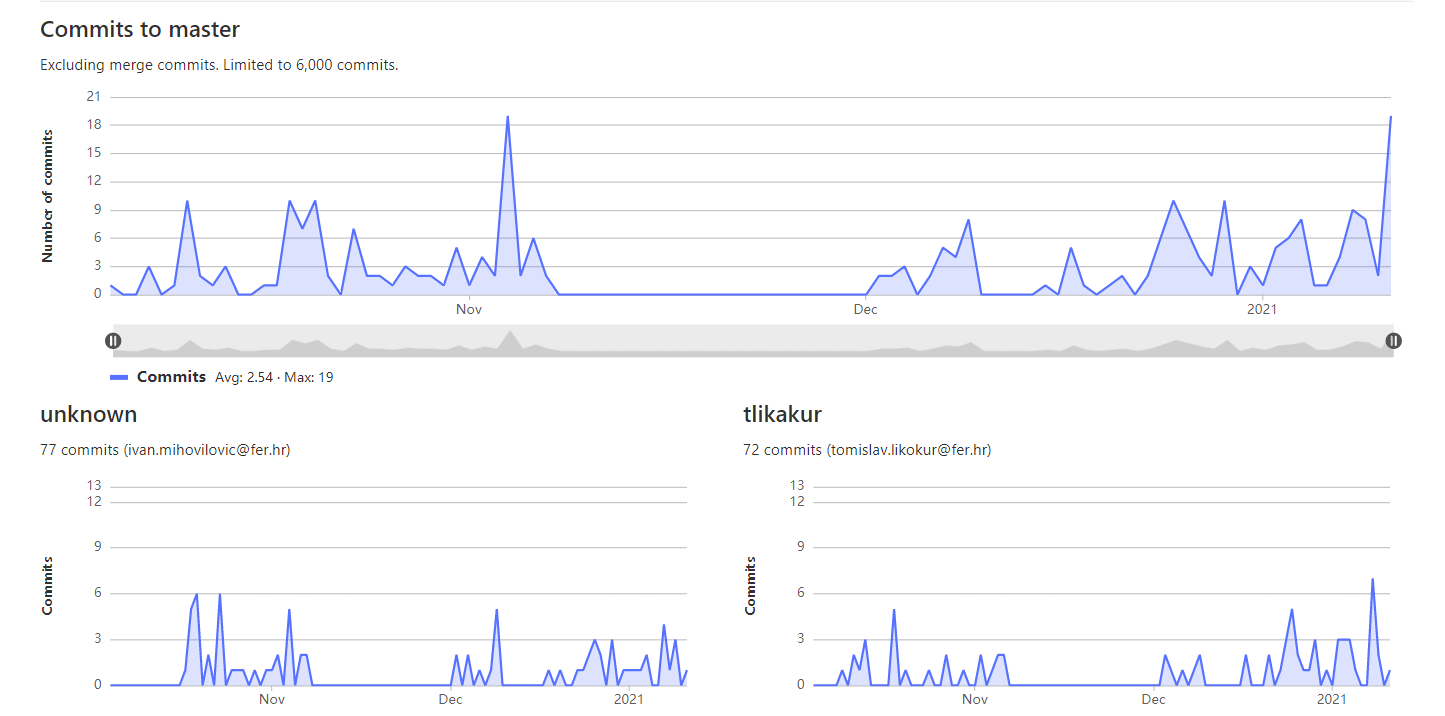
\includegraphics[scale=0.45]{slike/stat1.PNG} 
		 	\centering
		 	\caption{Statistika za granu master}
		 	\label{fig:stat1}%label mora biti drugaciji za svaku sliku
		 \end{figure}
	 	
	 	\begin{figure}[H]
	 		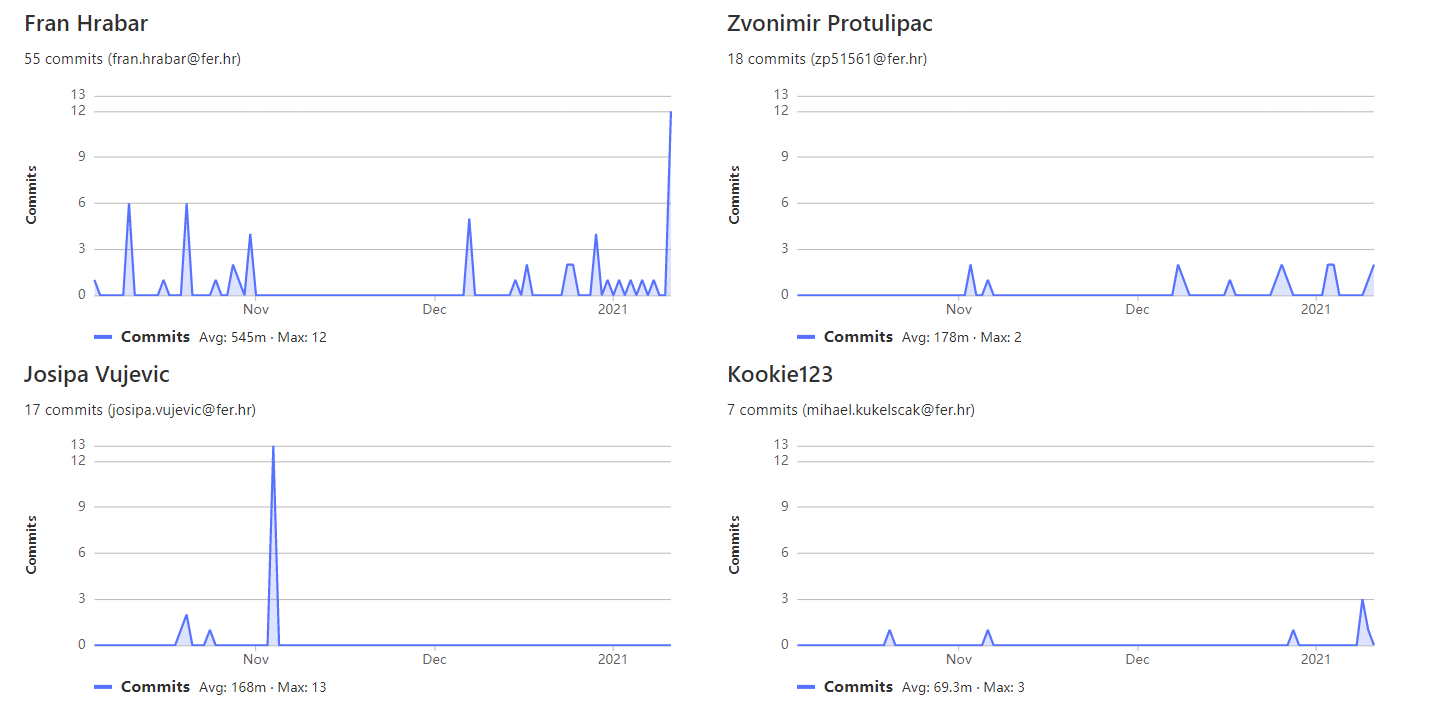
\includegraphics[scale=0.45]{slike/stat2.PNG} 
	 		\centering
	 		\caption{Statistika za granu master - nastavak}
	 		\label{fig:stat2}%label mora biti drugaciji za svaku sliku
	 	\end{figure}
 	
 		\begin{figure}[H]
 			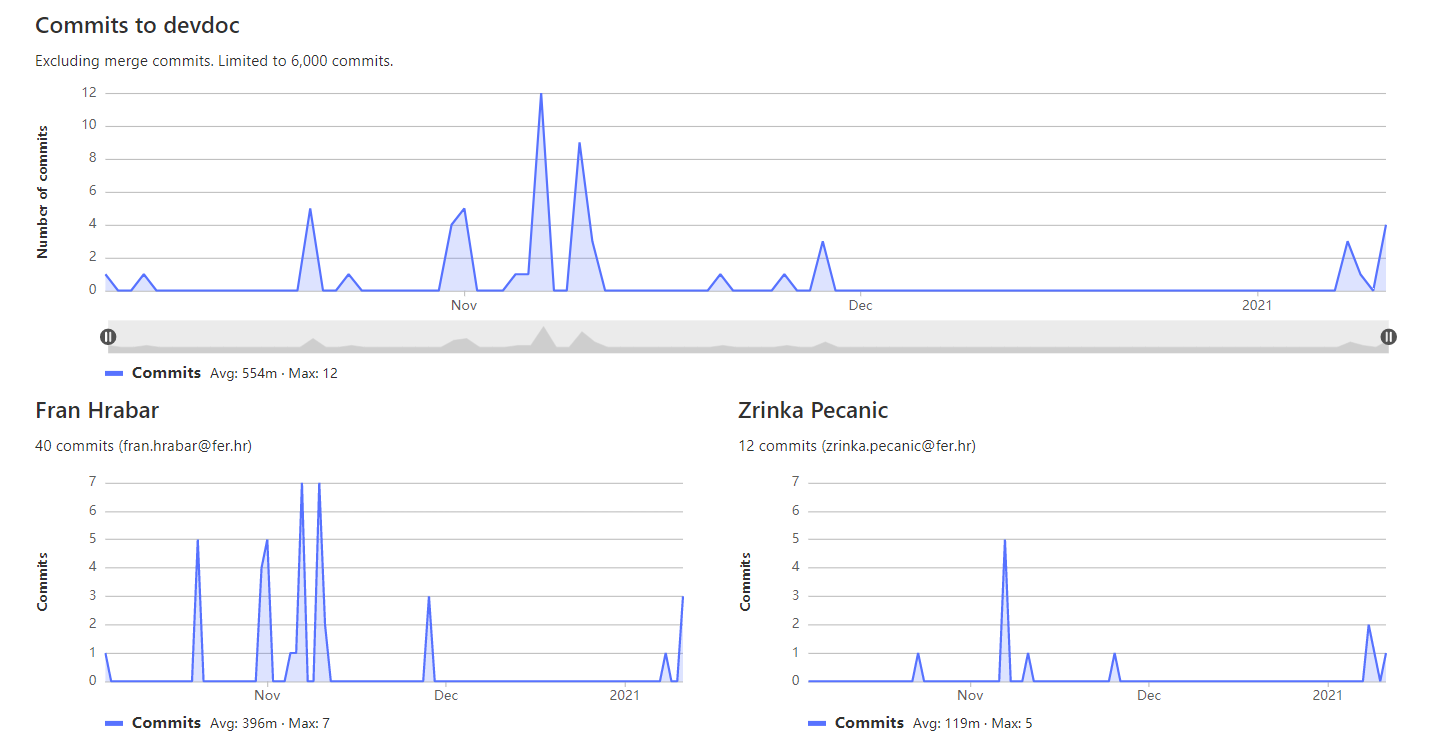
\includegraphics[scale=0.45]{slike/stat3.PNG} 
 			\centering
 			\caption{Statistika za granu devdoc}
 			\label{fig:stat3}%label mora biti drugaciji za svaku sliku
 		\end{figure}
 	
 		\begin{figure}[H]
 			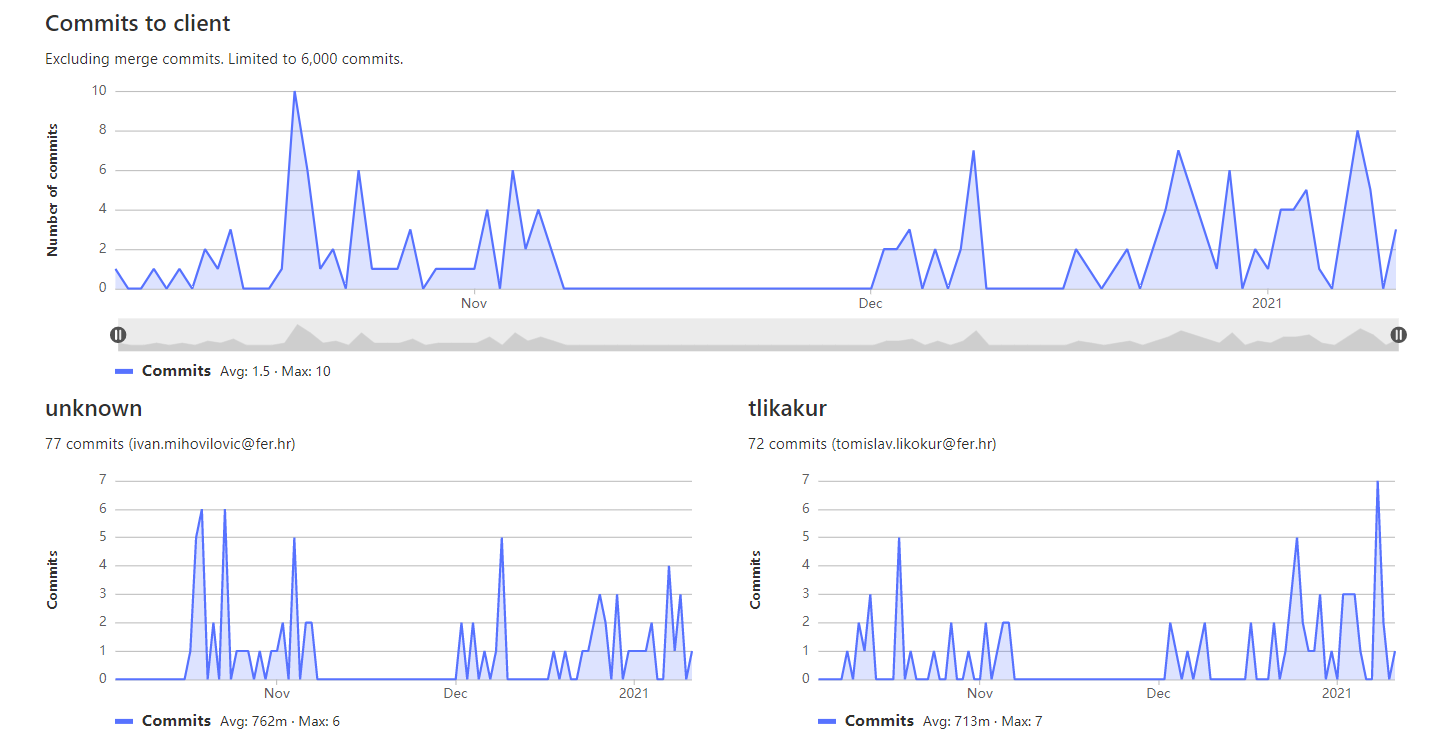
\includegraphics[scale=0.45]{slike/stat4.PNG} 
 			\centering
 			\caption{Statistika za granu client}
 			\label{fig:stat4}%label mora biti drugaciji za svaku sliku
 		\end{figure}
 	
 		 \begin{figure}[H]
 		 	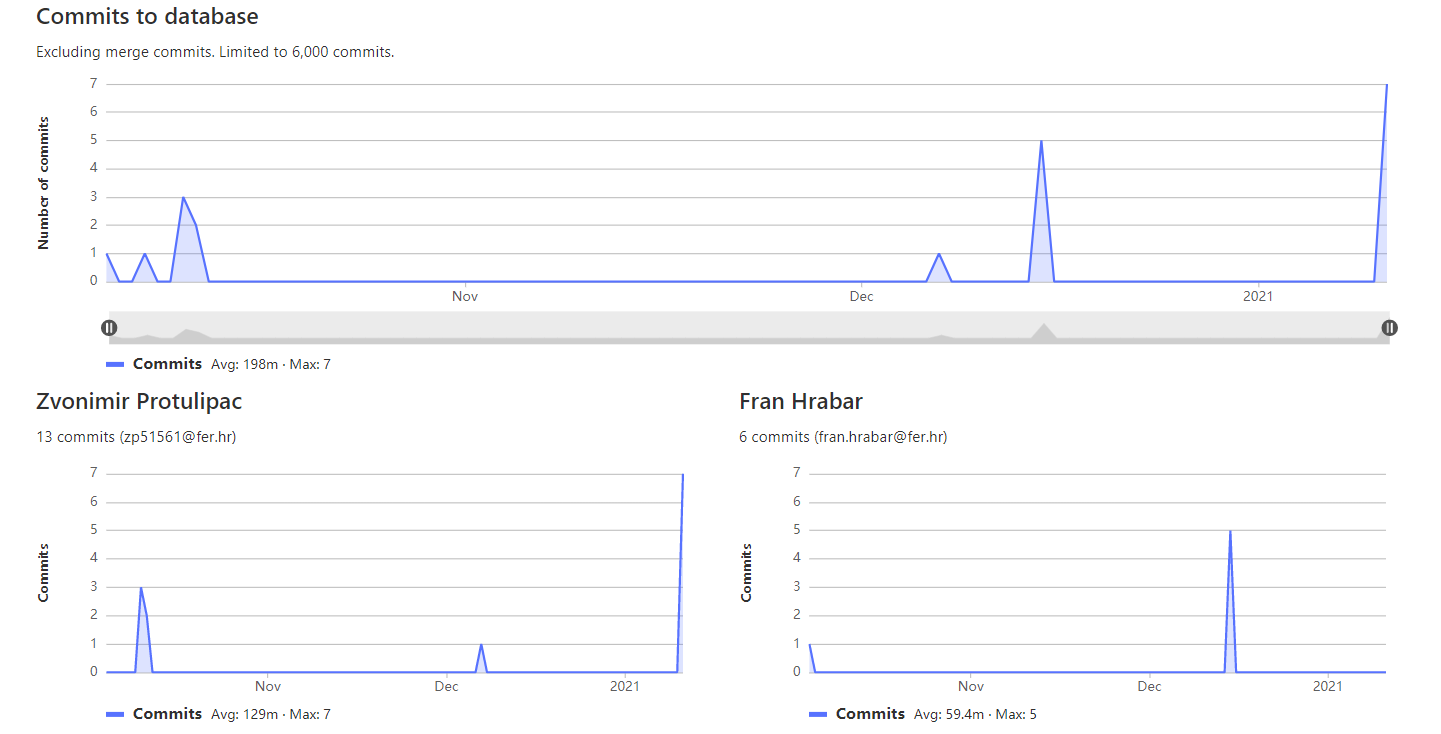
\includegraphics[scale=0.45]{slike/stat5.PNG} 
 		 	\centering
 		 	\caption{Statistika za granu database}
 		 	\label{fig:stat5}%label mora biti drugaciji za svaku sliku
 		 \end{figure}
	 
	%	\textbf{\textit{dio 2. revizije}}\\
		
		%\textit{Prenijeti dijagram pregleda promjena nad datotekama projekta. Potrebno je na kraju projekta generirane grafove s gitlaba prenijeti u ovo poglavlje dokumentacije. Dijagrami za vlastiti projekt se mogu preuzeti s gitlab.com stranice, u izborniku Repository, pritiskom na stavku Contributors.}
		
	